% Editable source for the filter pipeline and joint weak-order/length flowchart.
% Build from the repository root with:
%   & "$env:LOCALAPPDATA\Programs\MiKTeX\miktex\bin\x64\pdflatex.exe" `
%       -interaction=nonstopmode -halt-on-error `
%       -output-directory output\pdf docs\joint_solver_filter_flowchart.tex
\documentclass[10pt]{article}
\usepackage[T1]{fontenc}
\usepackage{lmodern}
\usepackage[a3paper,landscape,margin=8mm]{geometry}
\usepackage{xcolor}
\usepackage{tikz}
\usetikzlibrary{arrows.meta,backgrounds,calc,fit,positioning,shapes.geometric}
\pagestyle{empty}
\setlength{\parindent}{0pt}

\definecolor{ink}{HTML}{172033}
\definecolor{muted}{HTML}{5E6B82}
\definecolor{line}{HTML}{AAB7C9}
\definecolor{paper}{HTML}{F6F8FC}
\definecolor{data}{HTML}{E9EEF5}
\definecolor{domain}{HTML}{EEE8FF}
\definecolor{domainline}{HTML}{6D4AFF}
\definecolor{quotient}{HTML}{E6F0FF}
\definecolor{quotientline}{HTML}{2563EB}
\definecolor{necessary}{HTML}{E8F7EF}
\definecolor{necessaryline}{HTML}{15803D}
\definecolor{exact}{HTML}{E4F5F3}
\definecolor{exactline}{HTML}{047857}
\definecolor{resource}{HTML}{FFF3D8}
\definecolor{resourceline}{HTML}{B7791F}
\definecolor{numerical}{HTML}{FFF0E8}
\definecolor{numericalline}{HTML}{C2410C}
\definecolor{reject}{HTML}{FCE8E8}
\definecolor{rejectline}{HTML}{B42318}
\definecolor{joint}{HTML}{F2EAFE}
\definecolor{jointline}{HTML}{7C3AED}

\tikzset{
  flow/.style={-{Latex[length=3mm,width=2mm]},very thick,draw=ink},
  conditional/.style={-{Latex[length=2.6mm,width=1.8mm]},thick,draw=muted},
  sideflow/.style={-{Latex[length=2.6mm,width=1.8mm]},thick,dashed,draw=jointline},
  base/.style={rounded corners=2mm,very thick,align=left,inner sep=3mm,text=ink,font=\sffamily\footnotesize},
  dataBox/.style={base,draw=line,fill=data},
  domainBox/.style={base,draw=domainline,fill=domain},
  quotientBox/.style={base,draw=quotientline,fill=quotient},
  necessaryBox/.style={base,draw=necessaryline,fill=necessary},
  exactBox/.style={base,draw=exactline,fill=exact},
  resourceBox/.style={base,draw=resourceline,fill=resource},
  numericalBox/.style={base,draw=numericalline,fill=numerical},
  jointBox/.style={base,draw=jointline,fill=joint},
  rejectBox/.style={base,draw=rejectline,fill=reject},
  decision/.style={diamond,aspect=2.0,very thick,draw=ink,fill=white,align=center,inner sep=1.8mm,font=\sffamily\footnotesize},
  title/.style={font=\sffamily\bfseries\fontsize{20}{22}\selectfont,text=ink,anchor=west},
  subtitle/.style={font=\sffamily\fontsize{9}{11}\selectfont,text=muted,anchor=west},
  tag/.style={rounded corners=1mm,draw=line,fill=white,inner xsep=2mm,inner ysep=1mm,font=\sffamily\scriptsize,text=muted},
  smallnote/.style={font=\sffamily\scriptsize,text=muted,align=left},
}

\newcommand{\boxtitle}[2]{%
  {\color{#1}\bfseries #2}\par\vspace{1.2mm}%
}
\newcommand{\filterid}[1]{\texttt{#1}}

\begin{document}
\pagecolor{paper}

% ---------------------------------------------------------------------------
% Page 1: complete conditional sequence
% ---------------------------------------------------------------------------
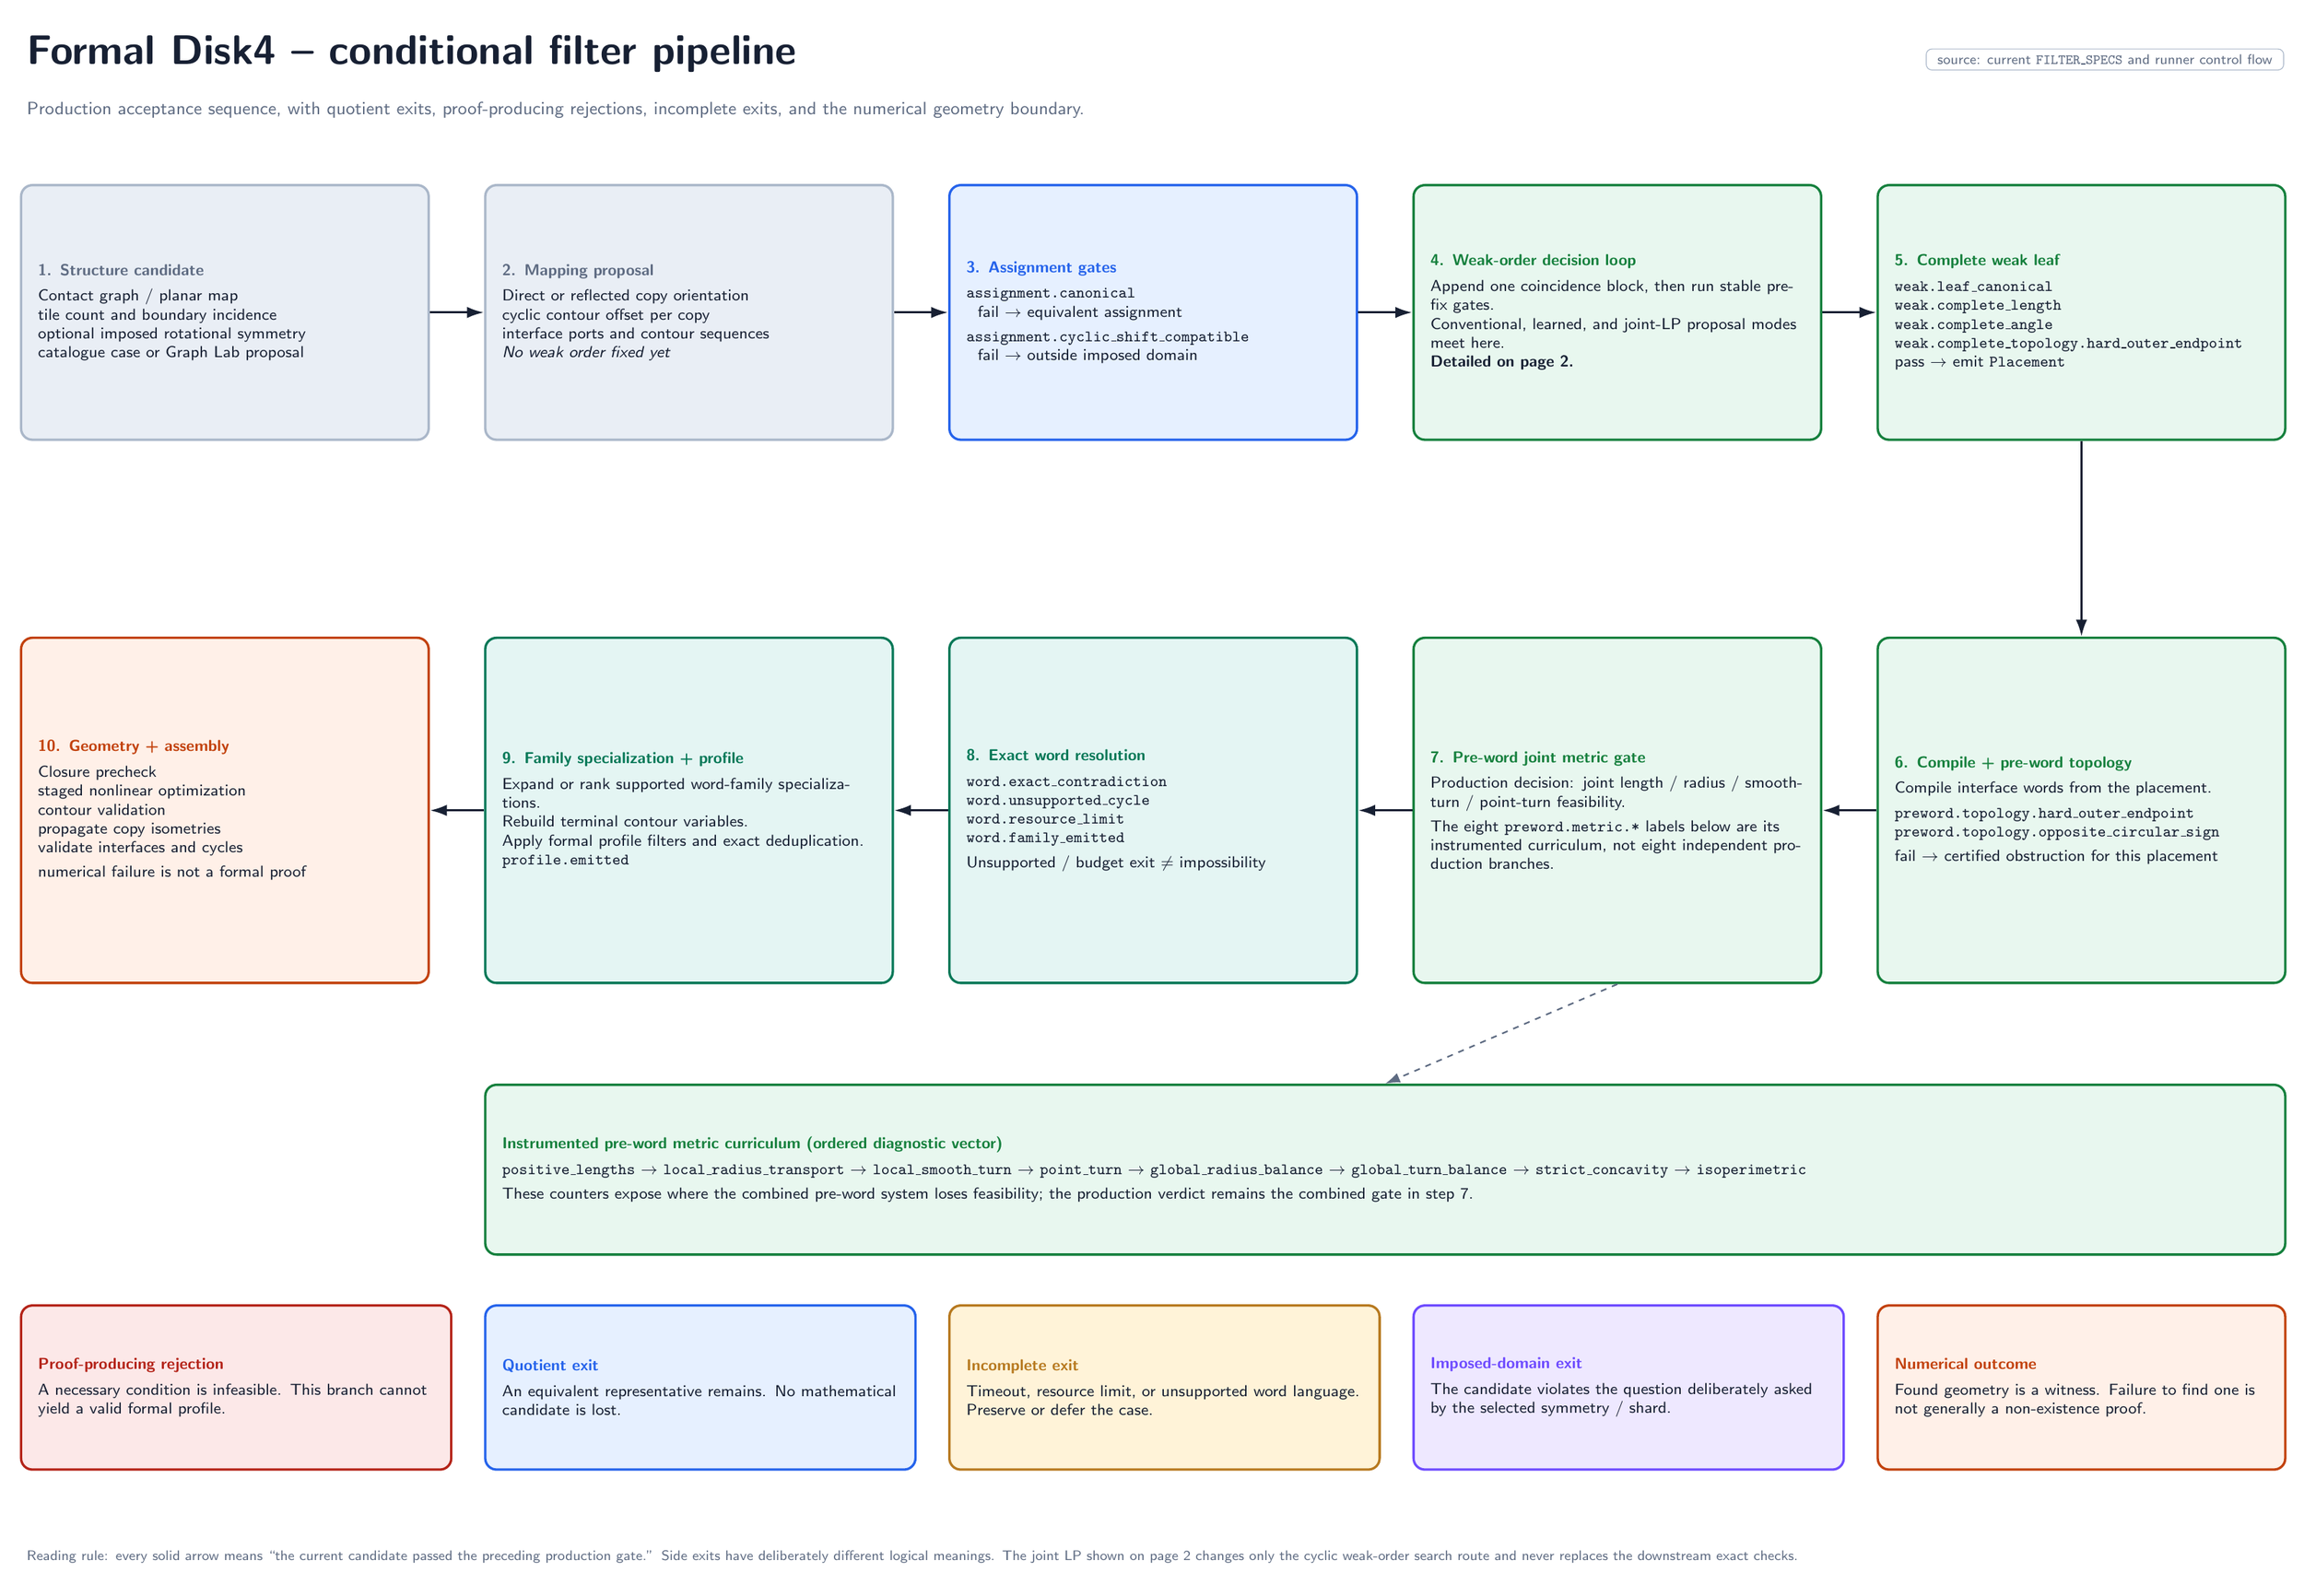
\begin{tikzpicture}[x=1mm,y=1mm]
  \path[use as bounding box] (0,0) rectangle (400,275);
  \node[title] at (0,269) {Formal Disk4 -- conditional filter pipeline};
  \node[subtitle] at (0,259) {Production acceptance sequence, with quotient exits, proof-producing rejections, incomplete exits, and the numerical geometry boundary.};
  \node[tag,anchor=east] at (400,268) {source: current \texttt{FILTER\_SPECS} and runner control flow};

  % First row, left to right.
  \node[dataBox,text width=66mm,minimum height=45mm,anchor=north west] (p1) at (0,246) {
    \boxtitle{muted}{1. Structure candidate}
    Contact graph / planar map\par
    tile count and boundary incidence\par
    optional imposed rotational symmetry\par
    catalogue case or Graph Lab proposal
  };

  \node[dataBox,text width=66mm,minimum height=45mm,anchor=north west] (p2) at (82,246) {
    \boxtitle{muted}{2. Mapping proposal}
    Direct or reflected copy orientation\par
    cyclic contour offset per copy\par
    interface ports and contour sequences\par
    \emph{No weak order fixed yet}
  };

  \node[quotientBox,text width=66mm,minimum height=45mm,anchor=north west] (p3) at (164,246) {
    \boxtitle{quotientline}{3. Assignment gates}
    \filterid{assignment.canonical}\par
    \hspace{2mm}fail $\rightarrow$ equivalent assignment\par\vspace{1mm}
    \filterid{assignment.cyclic\_shift\_compatible}\par
    \hspace{2mm}fail $\rightarrow$ outside imposed domain
  };

  \node[necessaryBox,text width=66mm,minimum height=45mm,anchor=north west] (p4) at (246,246) {
    \boxtitle{necessaryline}{4. Weak-order decision loop}
    Append one coincidence block, then run stable prefix gates.\par
    Conventional, learned, and joint-LP proposal modes meet here.\par
    \textbf{Detailed on page 2.}
  };

  \node[necessaryBox,text width=66mm,minimum height=45mm,anchor=north west] (p5) at (328,246) {
    \boxtitle{necessaryline}{5. Complete weak leaf}
    \filterid{weak.leaf\_canonical}\par
    \filterid{weak.complete\_length}\par
    \filterid{weak.complete\_angle}\par
    \filterid{weak.complete\_topology.hard\_outer\_endpoint}\par
    pass $\rightarrow$ emit \texttt{Placement}
  };

  \draw[flow] (p1.east) -- (p2.west);
  \draw[flow] (p2.east) -- (p3.west);
  \draw[flow] (p3.east) -- (p4.west);
  \draw[flow] (p4.east) -- (p5.west);

  % Second row, right to left.
  \node[necessaryBox,text width=66mm,minimum height=61mm,anchor=north west] (p6) at (328,166) {
    \boxtitle{necessaryline}{6. Compile + pre-word topology}
    Compile interface words from the placement.\par\vspace{1mm}
    \filterid{preword.topology.hard\_outer\_endpoint}\par
    \filterid{preword.topology.opposite\_circular\_sign}\par\vspace{1mm}
    fail $\rightarrow$ certified obstruction for this placement
  };

  \node[necessaryBox,text width=66mm,minimum height=61mm,anchor=north west] (p7) at (246,166) {
    \boxtitle{necessaryline}{7. Pre-word joint metric gate}
    Production decision: joint length / radius / smooth-turn / point-turn feasibility.\par\vspace{1mm}
    The eight \filterid{preword.metric.*} labels below are its instrumented curriculum, not eight independent production branches.
  };

  \node[exactBox,text width=66mm,minimum height=61mm,anchor=north west] (p8) at (164,166) {
    \boxtitle{exactline}{8. Exact word resolution}
    \filterid{word.exact\_contradiction}\par
    \filterid{word.unsupported\_cycle}\par
    \filterid{word.resource\_limit}\par
    \filterid{word.family\_emitted}\par\vspace{1mm}
    Unsupported / budget exit $\neq$ impossibility
  };

  \node[exactBox,text width=66mm,minimum height=61mm,anchor=north west] (p9) at (82,166) {
    \boxtitle{exactline}{9. Family specialization + profile}
    Expand or rank supported word-family specializations.\par
    Rebuild terminal contour variables.\par
    Apply formal profile filters and exact deduplication.\par
    \filterid{profile.emitted}
  };

  \node[numericalBox,text width=66mm,minimum height=61mm,anchor=north west] (p10) at (0,166) {
    \boxtitle{numericalline}{10. Geometry + assembly}
    Closure precheck\par
    staged nonlinear optimization\par
    contour validation\par
    propagate copy isometries\par
    validate interfaces and cycles\par\vspace{1mm}
    numerical failure is not a formal proof
  };

  \draw[flow] (p5.south) -- ++(0,-8) -| (p6.north);
  \draw[flow] (p6.west) -- (p7.east);
  \draw[flow] (p7.west) -- (p8.east);
  \draw[flow] (p8.west) -- (p9.east);
  \draw[flow] (p9.west) -- (p10.east);

  % The diagnostic decomposition of the actual preword metric gate.
  \node[necessaryBox,text width=312mm,minimum height=30mm,anchor=north west] (curriculum) at (82,87) {
    \boxtitle{necessaryline}{Instrumented pre-word metric curriculum (ordered diagnostic vector)}
    \filterid{positive\_lengths} $\rightarrow$
    \filterid{local\_radius\_transport} $\rightarrow$
    \filterid{local\_smooth\_turn} $\rightarrow$
    \filterid{point\_turn} $\rightarrow$
    \filterid{global\_radius\_balance} $\rightarrow$
    \filterid{global\_turn\_balance} $\rightarrow$
    \filterid{strict\_concavity} $\rightarrow$
    \filterid{isoperimetric}\par\vspace{1mm}
    These counters expose where the combined pre-word system loses feasibility; the production verdict remains the combined gate in step 7.
  };
  \draw[conditional,dashed] (p7.south) -- (curriculum.north);

  % Outcome semantics.
  \node[rejectBox,text width=70mm,minimum height=29mm,anchor=north west] (out1) at (0,48) {
    \boxtitle{rejectline}{Proof-producing rejection}
    A necessary condition is infeasible. This branch cannot yield a valid formal profile.
  };
  \node[quotientBox,text width=70mm,minimum height=29mm,anchor=north west] (out2) at (82,48) {
    \boxtitle{quotientline}{Quotient exit}
    An equivalent representative remains. No mathematical candidate is lost.
  };
  \node[resourceBox,text width=70mm,minimum height=29mm,anchor=north west] (out3) at (164,48) {
    \boxtitle{resourceline}{Incomplete exit}
    Timeout, resource limit, or unsupported word language. Preserve or defer the case.
  };
  \node[domainBox,text width=70mm,minimum height=29mm,anchor=north west] (out4) at (246,48) {
    \boxtitle{domainline}{Imposed-domain exit}
    The candidate violates the question deliberately asked by the selected symmetry / shard.
  };
  \node[numericalBox,text width=66mm,minimum height=29mm,anchor=north west] (out5) at (328,48) {
    \boxtitle{numericalline}{Numerical outcome}
    Found geometry is a witness. Failure to find one is not generally a non-existence proof.
  };

  \node[smallnote,anchor=south west,text width=397mm] at (0,1) {
    Reading rule: every solid arrow means ``the current candidate passed the preceding production gate.'' Side exits have deliberately different logical meanings. The joint LP shown on page 2 changes only the cyclic weak-order search route and never replaces the downstream exact checks.
  };
\end{tikzpicture}

\newpage

% ---------------------------------------------------------------------------
% Page 2: detailed joint weak-order and length branch
% ---------------------------------------------------------------------------
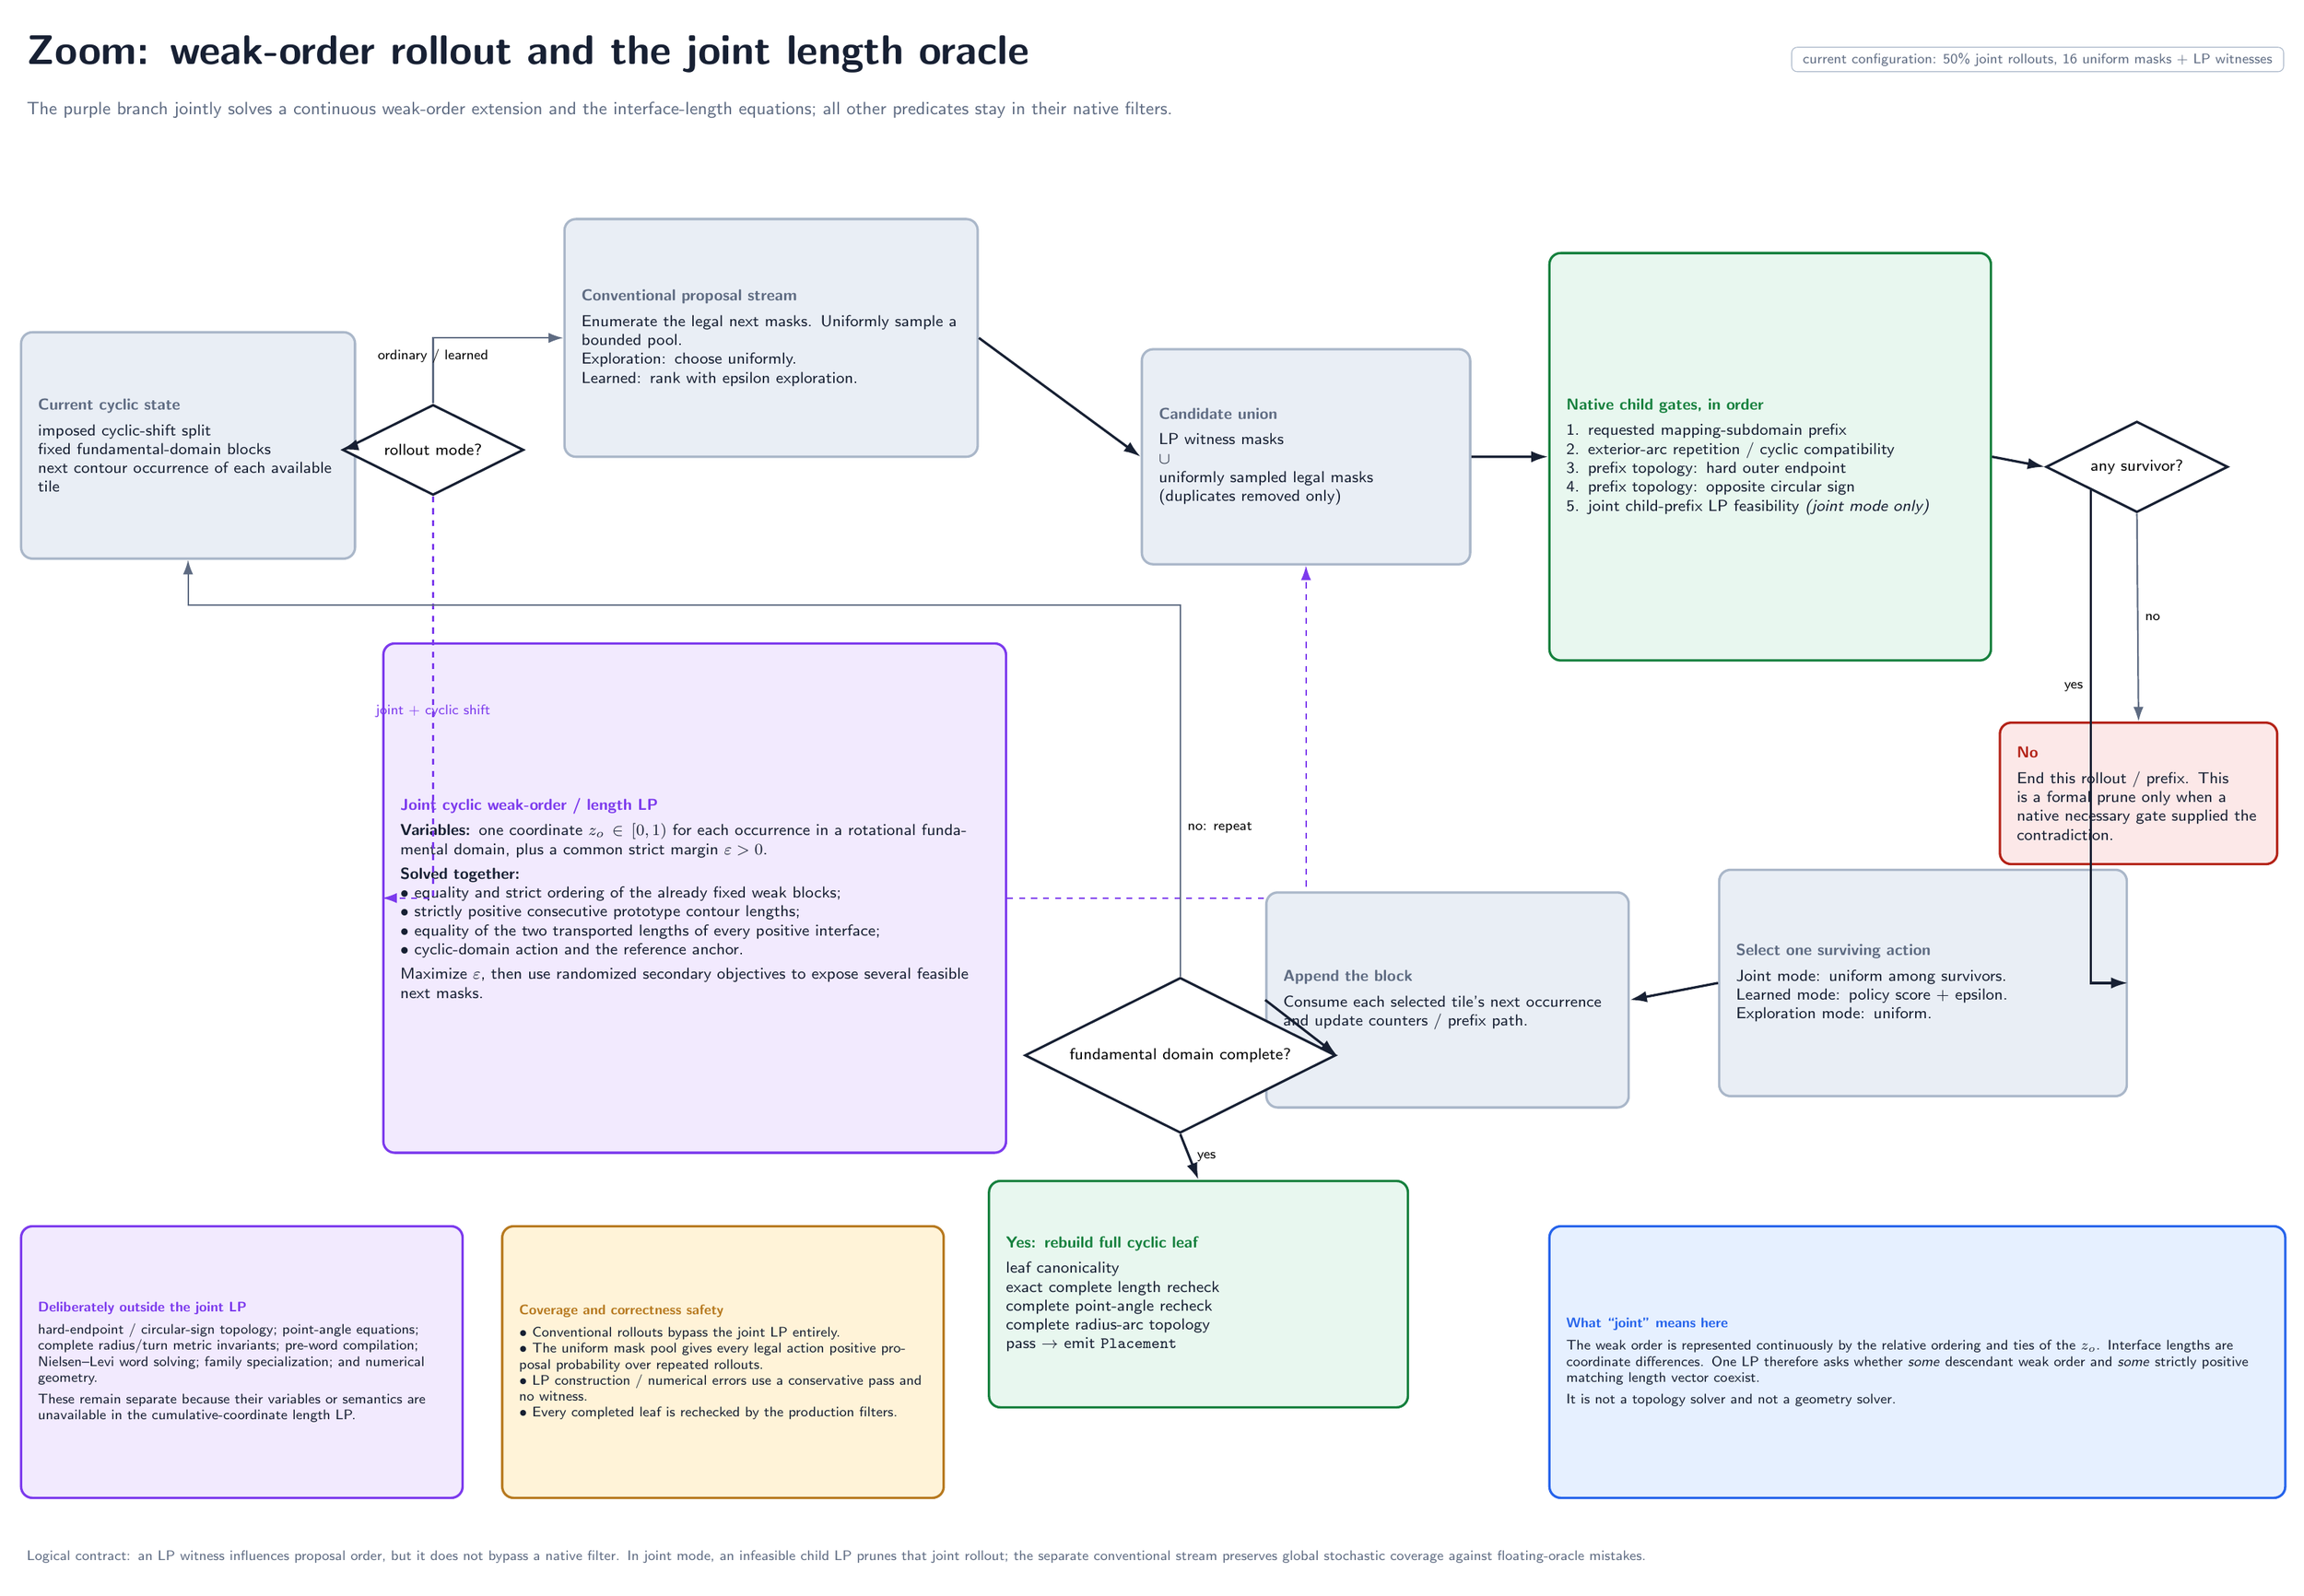
\begin{tikzpicture}[x=1mm,y=1mm]
  \path[use as bounding box] (0,0) rectangle (400,275);
  \node[title] at (0,269) {Zoom: weak-order rollout and the joint length oracle};
  \node[subtitle] at (0,259) {The purple branch jointly solves a continuous weak-order extension and the interface-length equations; all other predicates stay in their native filters.};
  \node[tag,anchor=east] at (400,268) {current configuration: 50\% joint rollouts, 16 uniform masks + LP witnesses};

  \node[dataBox,text width=53mm,minimum height=40mm,anchor=north west] (state) at (0,220) {
    \boxtitle{muted}{Current cyclic state}
    imposed cyclic-shift split\par
    fixed fundamental-domain blocks\par
    next contour occurrence of each available tile
  };

  \node[decision] (mode) at (73,199) {rollout\ mode?};
  \draw[flow] (state.east) -- (mode.west);

  \node[dataBox,text width=67mm,minimum height=42mm,anchor=north west] (ordinary) at (96,240) {
    \boxtitle{muted}{Conventional proposal stream}
    Enumerate the legal next masks. Uniformly sample a bounded pool.\par
    Exploration: choose uniformly.\par
    Learned: rank with epsilon exploration.
  };

  \node[jointBox,text width=104mm,minimum height=90mm,anchor=north west] (jointlp) at (64,165) {
    \boxtitle{jointline}{Joint cyclic weak-order / length LP}
    \textbf{Variables:} one coordinate $z_o\in[0,1)$ for each occurrence in a rotational fundamental domain, plus a common strict margin $\varepsilon>0$.\par\vspace{1mm}
    \textbf{Solved together:}\par
    $\bullet$ equality and strict ordering of the already fixed weak blocks;\par
    $\bullet$ strictly positive consecutive prototype contour lengths;\par
    $\bullet$ equality of the two transported lengths of every positive interface;\par
    $\bullet$ cyclic-domain action and the reference anchor.\par\vspace{1mm}
    Maximize $\varepsilon$, then use randomized secondary objectives to expose several feasible next masks.
  };

  \draw[conditional] (mode.north) |- node[pos=0.25,above,font=\sffamily\scriptsize] {ordinary / learned} (ordinary.west);
  \draw[sideflow] (mode.south) |- node[pos=0.25,below,font=\sffamily\scriptsize,text=jointline] {joint + cyclic shift} (jointlp.west);

  \node[dataBox,text width=52mm,minimum height=38mm,anchor=north west] (merge) at (198,217) {
    \boxtitle{muted}{Candidate union}
    LP witness masks\par
    $\cup$\par
    uniformly sampled legal masks\par
    (duplicates removed only)
  };
  \draw[flow] (ordinary.east) -- (merge.west);
  \draw[sideflow] (jointlp.east) -| (merge.south);

  \node[necessaryBox,text width=72mm,minimum height=72mm,anchor=north west] (gates) at (270,234) {
    \boxtitle{necessaryline}{Native child gates, in order}
    1. requested mapping-subdomain prefix\par
    2. exterior-arc repetition / cyclic compatibility\par
    3. prefix topology: hard outer endpoint\par
    4. prefix topology: opposite circular sign\par
    5. joint child-prefix LP feasibility \emph{(joint mode only)}
  };
  \draw[flow] (merge.east) -- (gates.west);

  \node[decision] (survive) at (374,196) {any\ survivor?};
  \draw[flow] (gates.east) -- (survive.west);

  \node[rejectBox,text width=43mm,minimum height=25mm,anchor=north east] (dead) at (399,151) {
    \boxtitle{rejectline}{No}
    End this rollout / prefix. This is a formal prune only when a native necessary gate supplied the contradiction.
  };
  \draw[conditional] (survive.south) -- node[right,font=\sffamily\scriptsize] {no} (dead.north);

  \node[dataBox,text width=66mm,minimum height=40mm,anchor=north west] (select) at (300,125) {
    \boxtitle{muted}{Select one surviving action}
    Joint mode: uniform among survivors.\par
    Learned mode: policy score + epsilon.\par
    Exploration mode: uniform.
  };
  \draw[flow] (survive.south west) |- node[pos=0.2,left,font=\sffamily\scriptsize] {yes} (select.east);

  \node[dataBox,text width=58mm,minimum height=38mm,anchor=north west] (append) at (220,121) {
    \boxtitle{muted}{Append the block}
    Consume each selected tile's next occurrence and update counters / prefix path.
  };
  \draw[flow] (select.west) -- (append.east);

  \node[decision] (complete) at (205,92) {fundamental domain complete?};
  \draw[flow] (append.west) -- (complete.east);
  \draw[conditional] (complete.north) |- node[pos=0.2,right,font=\sffamily\scriptsize] {no: repeat} ($(state.south)+(0,-8)$) -- (state.south);

  \node[necessaryBox,text width=68mm,minimum height=40mm,anchor=north west] (leaf) at (171,70) {
    \boxtitle{necessaryline}{Yes: rebuild full cyclic leaf}
    leaf canonicality\par
    exact complete length recheck\par
    complete point-angle recheck\par
    complete radius-arc topology\par
    pass $\rightarrow$ emit \texttt{Placement}
  };
  \draw[flow] (complete.south) -- node[right,font=\sffamily\scriptsize] {yes} (leaf.north);

  \node[jointBox,text width=72mm,minimum height=48mm,anchor=north west,font=\sffamily\scriptsize] (notjoint) at (0,62) {
    \boxtitle{jointline}{Deliberately outside the joint LP}
    hard-endpoint / circular-sign topology; point-angle equations; complete radius/turn metric invariants; pre-word compilation; Nielsen--Levi word solving; family specialization; and numerical geometry.\par\vspace{1mm}
    These remain separate because their variables or semantics are unavailable in the cumulative-coordinate length LP.
  };

  \node[resourceBox,text width=72mm,minimum height=48mm,anchor=north west,font=\sffamily\scriptsize] (safety) at (85,62) {
    \boxtitle{resourceline}{Coverage and correctness safety}
    $\bullet$ Conventional rollouts bypass the joint LP entirely.\par
    $\bullet$ The uniform mask pool gives every legal action positive proposal probability over repeated rollouts.\par
    $\bullet$ LP construction / numerical errors use a conservative pass and no witness.\par
    $\bullet$ Every completed leaf is rechecked by the production filters.
  };

  \node[quotientBox,text width=124mm,minimum height=48mm,anchor=north west,font=\sffamily\scriptsize] (meaning) at (270,62) {
    \boxtitle{quotientline}{What ``joint'' means here}
    The weak order is represented continuously by the relative ordering and ties of the $z_o$. Interface lengths are coordinate differences. One LP therefore asks whether \emph{some} descendant weak order and \emph{some} strictly positive matching length vector coexist.\par\vspace{1mm}
    It is not a topology solver and not a geometry solver.
  };

  \node[smallnote,anchor=south west,text width=397mm] at (0,1) {
    Logical contract: an LP witness influences proposal order, but it does not bypass a native filter. In joint mode, an infeasible child LP prunes that joint rollout; the separate conventional stream preserves global stochastic coverage against floating-oracle mistakes.
  };
\end{tikzpicture}

\end{document}
